% -----------------------------------------------------------------------------
%   Arquivo: ./02-elementos-textuais/introducao.tex
% -----------------------------------------------------------------------------



\chapter{Introdução}
\label{chap:introducao}

Edite e coloque aqui o seu texto introdutório do artigo.

A introdução deverá apresentar uma visão de conjunto do trabalho a ser realizado, com o apoio da literatura, situando-o no contexto do estado da arte da área científica específica, sua relevância no contexto da área inserida e sua importância específica para o avanço do conhecimento.

Deve ser dado destaque às contribuições efetivas do trabalho e sua relevância para a área de pesquisa.

É uma boa prática iniciar cada novo capítulo com uma breve texto introdutório (tipicamente, dois ou três parágrafos) que deve deixar claro o quê será discutido no capítulo, bem como a organização do capítulo. Também servirá ao propósito de "amarrar"{} ou "alinhavar"{}  o conteúdo deste capítulo com o conteúdo do capítulo imediatamente anterior - neste caso, contando  com o texto da seção de "Considerações finais"{}  do capítulo anterior.



\section{Leia esta seção antes de começar }
\label{sec:antesleiame}

Este documento é um \emph{template} \LaTeX{} que adaptado de Borges et. al., para ser utilizado em trabalho simples de mestrado e doutorado com conformidade as regras da ABNT. 

Há vários elementos do documento que sofrem conversão minúsculas/maiúsculas - por exemplo o conteúdo dos arquivos {\ttfamily .bib}, {\ttfamily capa.tex} e {\ttfamily folhaRosto.tex}, além de títulos de capítulos, seções, etc.. Para estes elementos, pelo menos, não acentue diretamente as palavras, use os comandos relacionados na \autoref{fig:acentosLatex}.

\begin{figure}[!htb]
	\centering
	\caption{Comandos para acentuação no \LaTeX}
	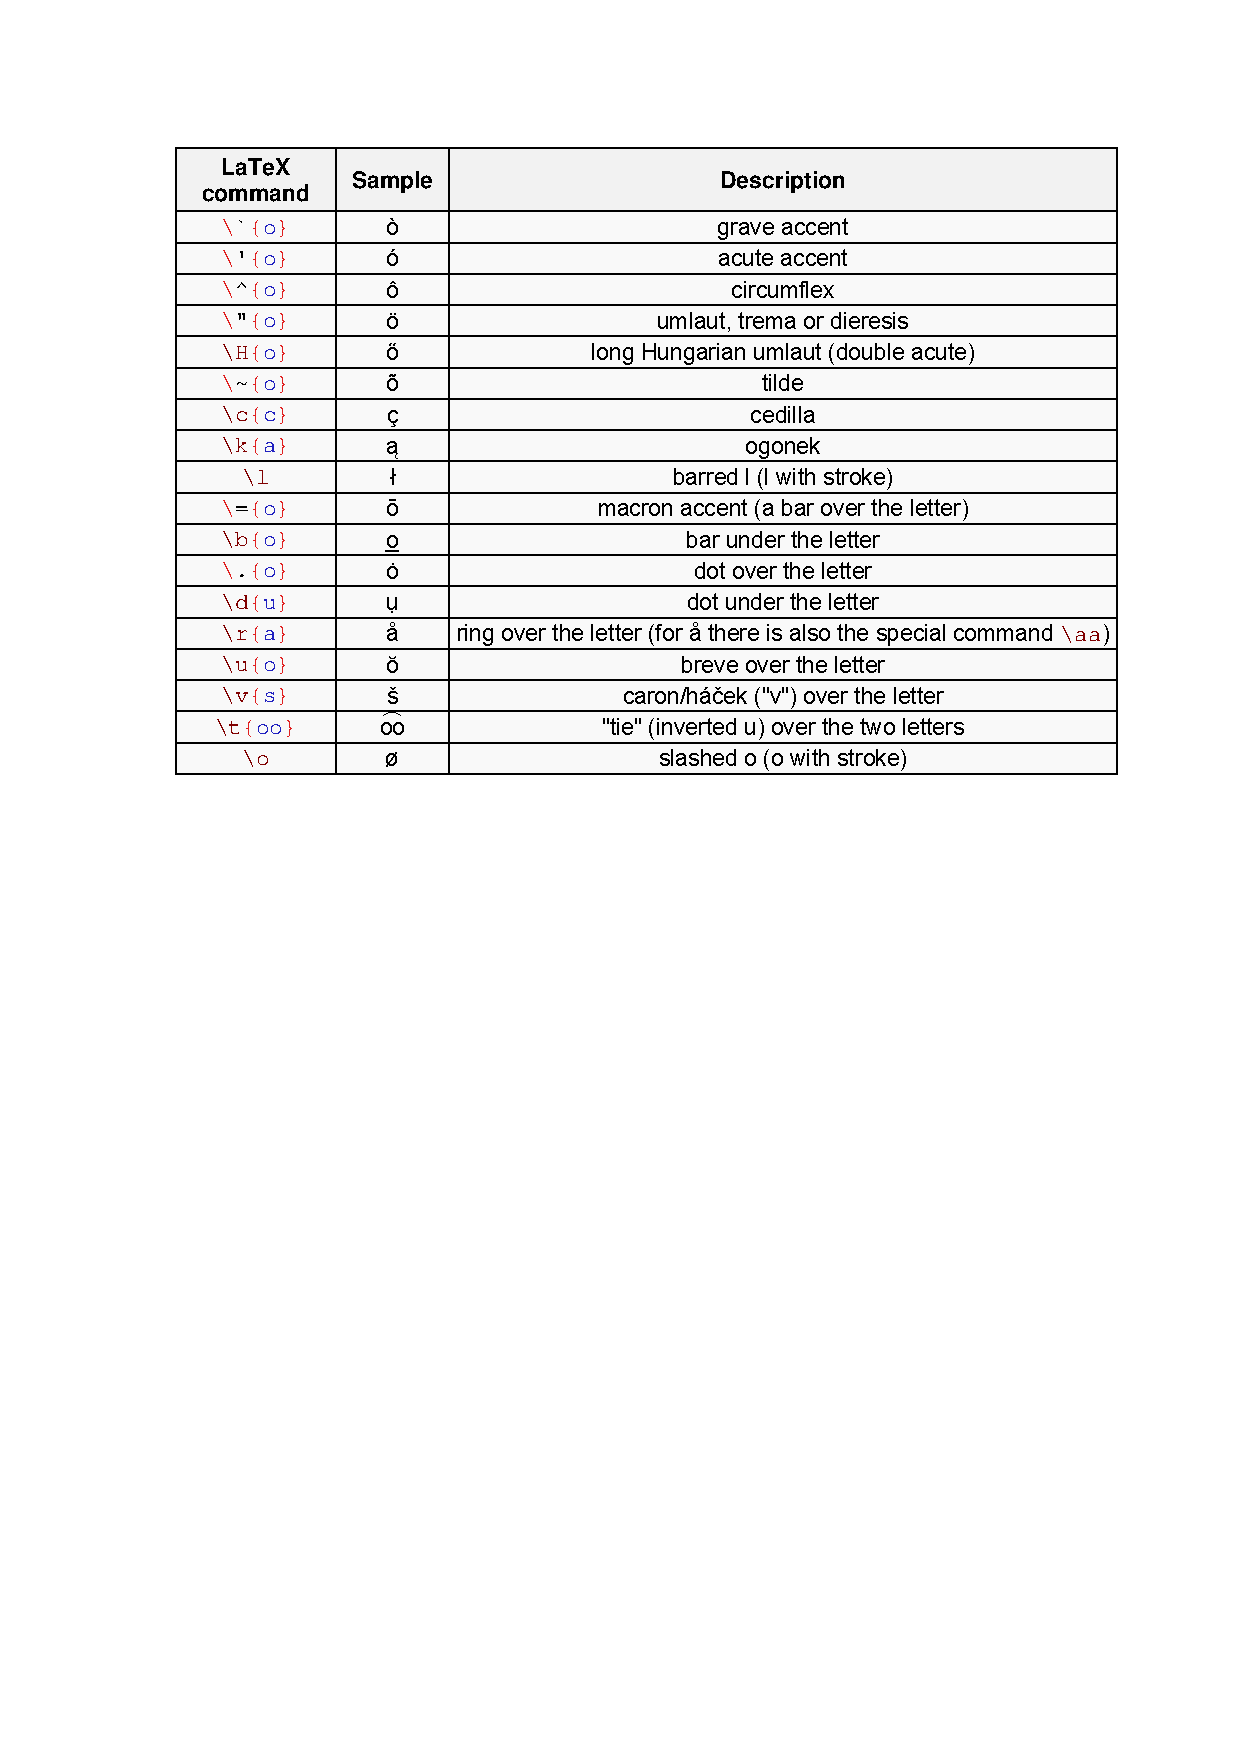
\includegraphics[width=0.8\textwidth]{./04-figuras/acentosLatex}
	\fonte{\href{http://en.wikibooks.org/wiki/LaTeX/Special_Characters}{http://en.wikibooks.org/wiki/LaTeX/Special\underline{ }Characters}}
	\label{fig:acentosLatex}
\end{figure}


Para a compilação de arquivos \TeX{} ou \LaTeX{} veja os comandos apresentados na \autoref{fig:comanCompilaTex}.


\begin{figure}[!htb]
	\centering
	\caption{Comandos para compilação de arquivos \TeX{} ou \LaTeX}
	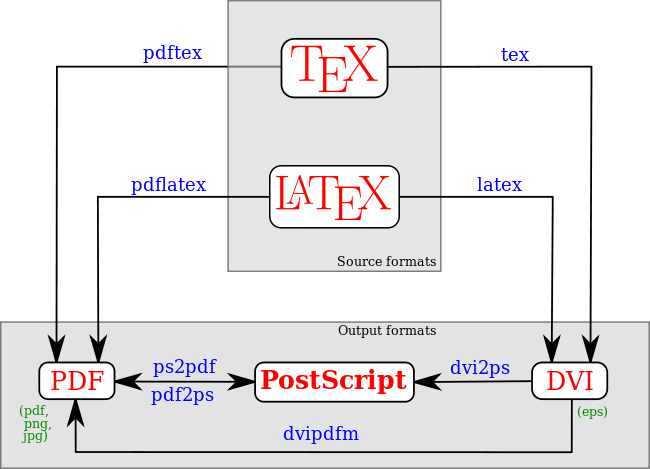
\includegraphics[width=0.8\textwidth]{./04-figuras/ComandosCompilacaoTex}
	\fonte{\href{http://en.wikibooks.org/wiki/LaTeX/Basics}{http://en.wikibooks.org/wiki/LaTeX/Basics}}
	\label{fig:comanCompilaTex}
\end{figure}


A compilação para gerar um arquivo no formato pdf, incluindo corretamente as referências bibliográficas, deve ser realizada em quatro passos:

\begin{compactitem}
	\item \textbf{pdflatex} \verb|meuTrabalhoAcademico.tex|    -> gera um pdf, porém sem as referências, apenas indicando-as
	\item \textbf{bibtex} \verb|meuTrabalhoAcademico.tex|	-> varre o arquivo myrefs.bib e busca pelas referências utilizadas
	\item \textbf{pdflatex} \verb|meuTrabalhoAcademico.tex|	-> insere as referências e chamadas nos locais apropriados
	\item \textbf{pdflatex} \verb|meuTrabalhoAcademico.tex|	-> faz a compilação final, verificando tudo
\end{compactitem}

Alternativamente, poderá ser utilizado o comando \verb|makefile|, disponível na mesma pasta onde está o arquivo principal \verb|meuTrabalhoAcademico.tex|, que faz exatamente o mesmo que os quatro comandos supramencionados. No entanto atente para o fato de que , se você alterar o nome do arquivo \verb|meuTrabalhoAcademico.tex|, deverá também editar o arquivo \verb|makefile| para alterá-lo do mesmo modo.

\section{Justificativa}
\label{sec:justificativa}

Blá blá blá .... 

